\chapter{Implementing the SoC}
\minitoc
\newpage

\setcounter{secnumdepth}{0} % Set the section counter to 0 so next section is not counted in toc
% ----------------------- Introduction ----------------------- %
\section{Introduction}
In this chapter, we will discuss the implementation of the Security Operation Center (SoC) that we designed in the previous chapter.
We will use Security Onion for the main center of operations and GNS3 to emulate the network environment.

\setcounter{secnumdepth}{2} % Resume counting the sections for the toc with a depth of 2 (Sections and sub-sections)
% ----------------------------------- SECTIONS (v) ----------------------------------- %
% ----------------------- Setting up the Network Environment ----------------------- %
\section{Setting up the Network Environment}
To start it off, we created a network topology in GNS3 that includes a pfSense firewall, acting as the gateway to the network, and multiple endpoints and servers as shown in the figure below.
The internet is simulated using a cloud node in GNS3 and it will just connect to the local network though a virtual bridge.

\begin{figure}[H]
    \centering
    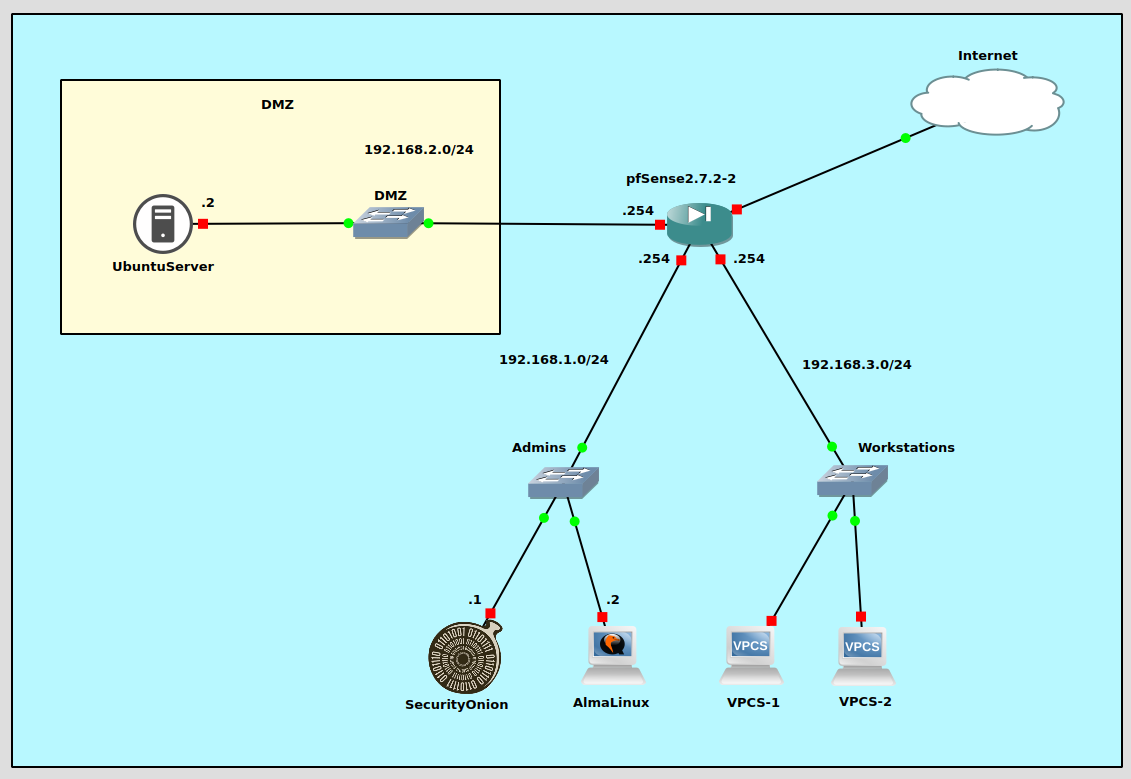
\includegraphics[width=1\textwidth]{src/assets/images/gns3-topology.png}
    \caption{Network Topology in GNS3}
\end{figure}

% ----------------------- Security Onion ----------------------- %
\section{Security Onion}
Security Onion is a free and open-source Linux distribution for threat hunting, enterprise security monitoring, and log management.
It includes Elasticsearch, Logstash, Kibana, Snort, Suricata, Zeek, Wazuh, TheHive, CyberChef, and many other security tools.

\begin{figure}[H]
    \centering
    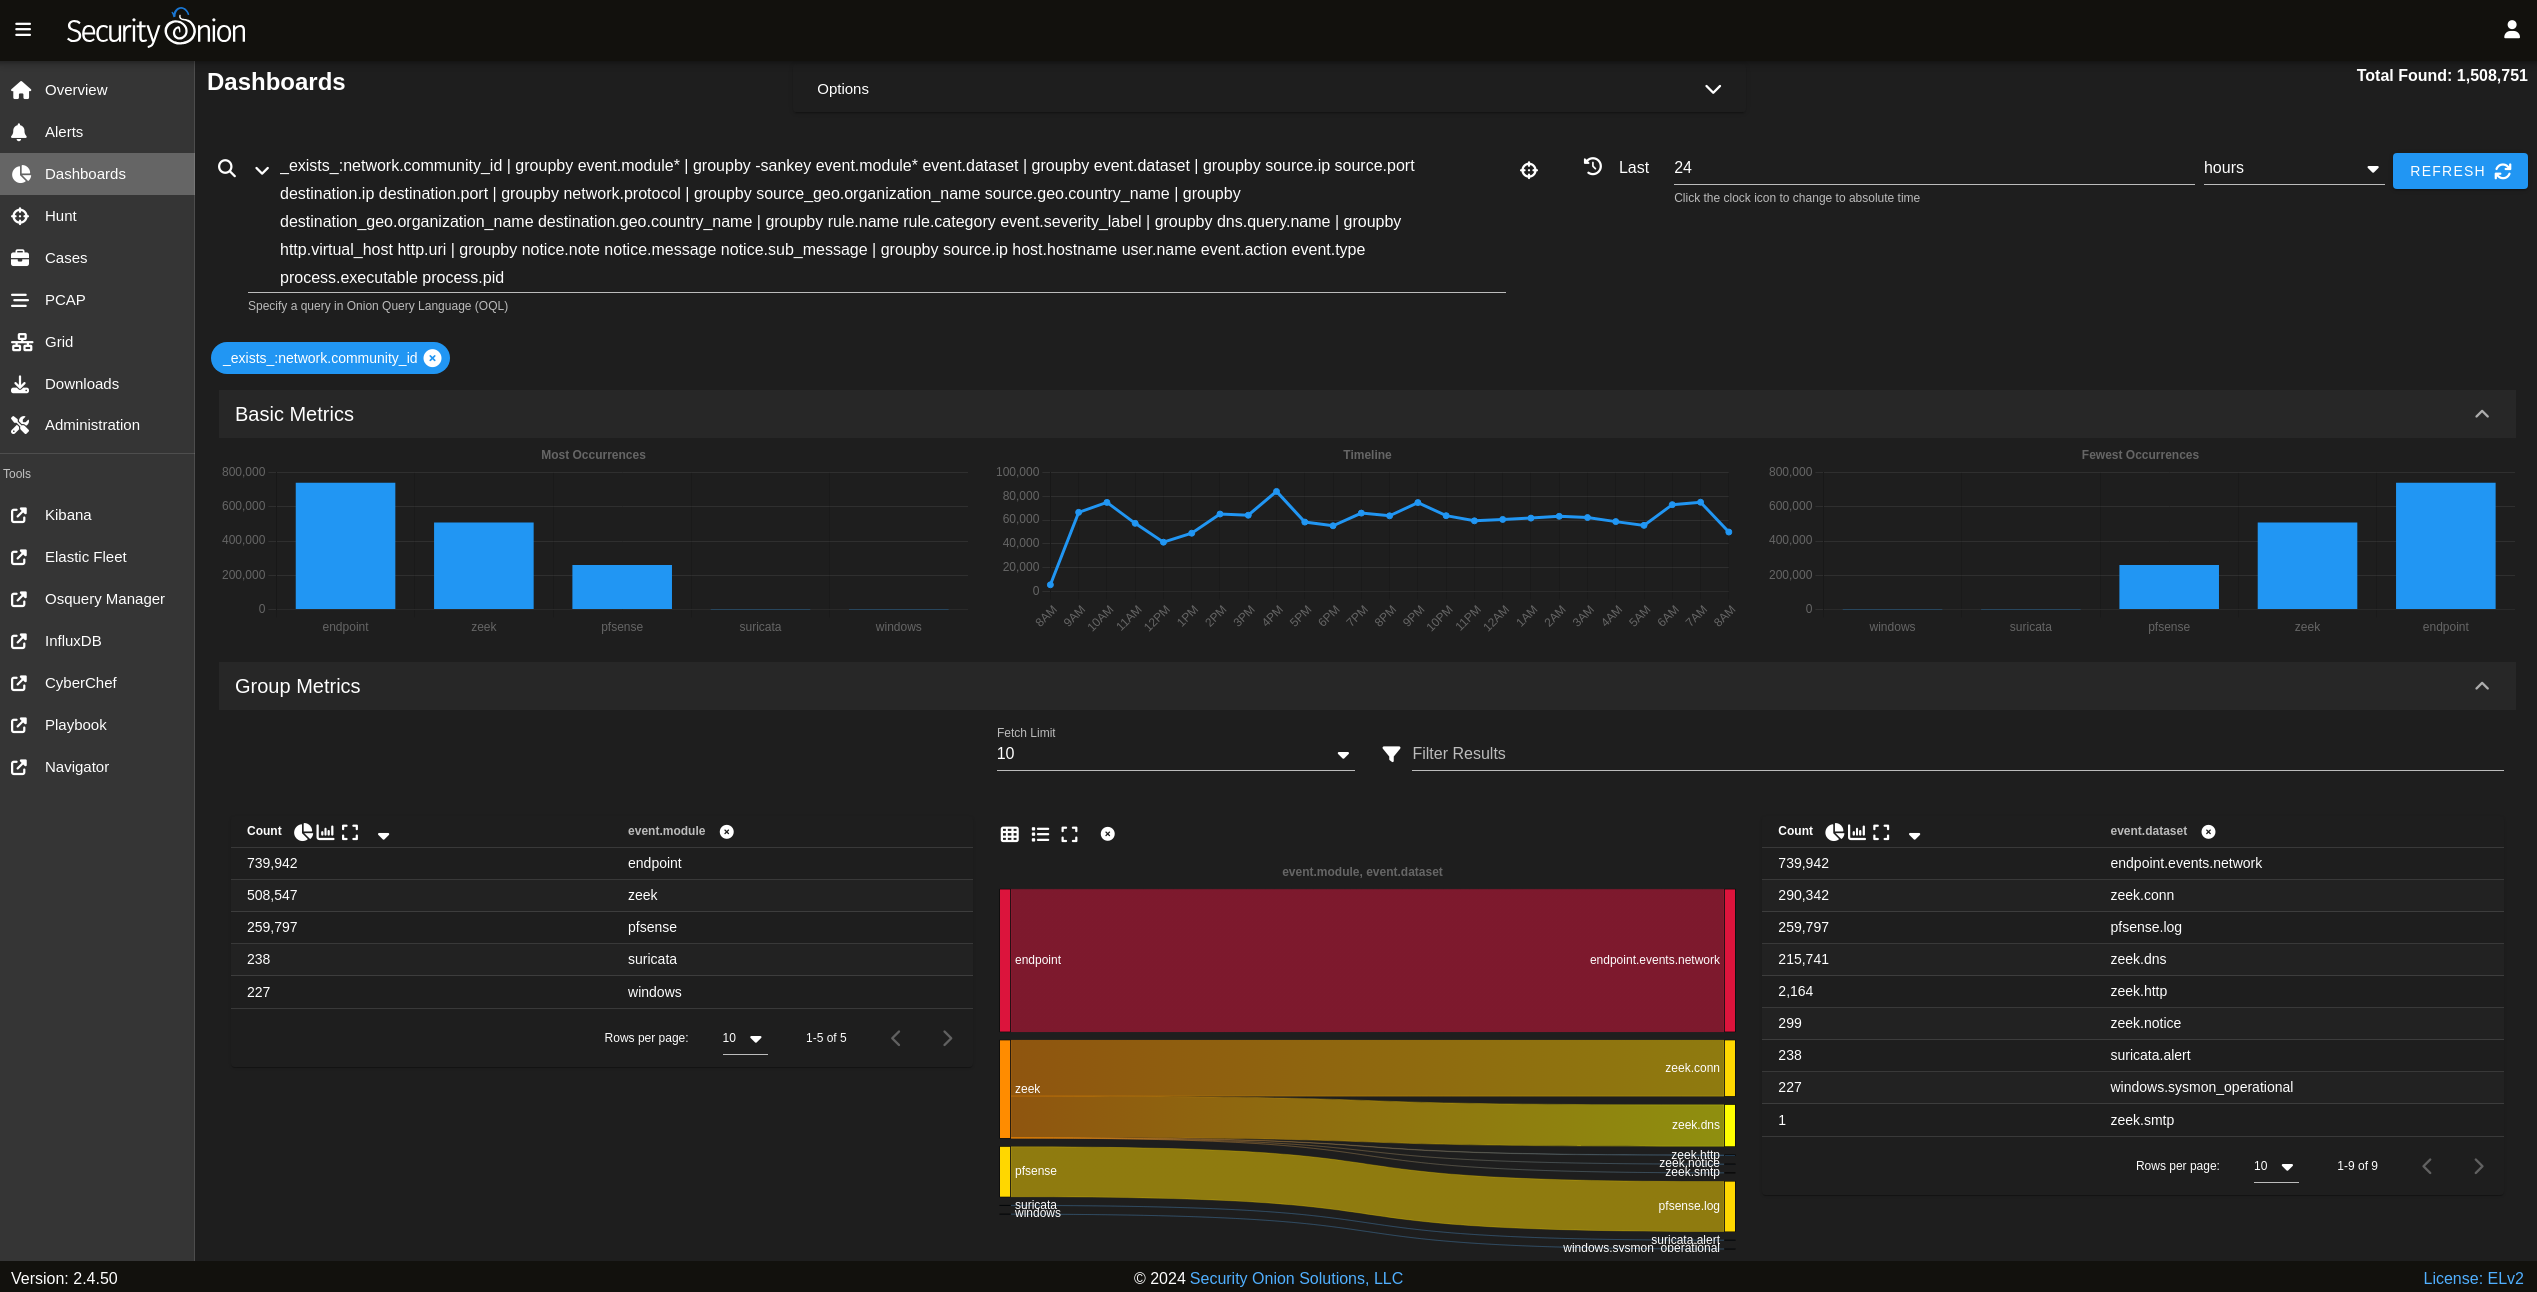
\includegraphics[width=1\textwidth]{src/assets/images/security-onion-sample.png}
    \caption{Example of Security Onion Dashboard}
\end{figure}

This is the brain of our SoC, where all the data from the network will be collected, analyzed, and responded to.

% ----------------------- Training the personnel ----------------------- %
\section{Training the personnel}
Of course, since this is an academic project no real training was provided, but in a proper SoC, training and skills development are crucial for the team to be able to effectively monitor and respond to security incidents.

This step did however manifest in the form of learning how to properly use Security Onion via the official documentation and online tutorials.

% ----------------------- Technologies ----------------------- %
\section{Technologies}
This part is reserved for the presentation of all of the software used in the realization of the project and includes but is not limited to; programming languages, frameworks, technologies, etc...

\medskip
For a comparative analysis on some of our choices, see \textbf {Chapter 2: State of the art}.

\begin{itemize}
    \item \textbf{Graphical Network Simulator 3 (GNS3):} \newline The most popular network software emulator, used to emulate network devices and create any network topology \newline
          \begin{minipage}{\linewidth}
              \centering
              
\includegraphics[width=3.5cm]{src/assets/logos/gns3_94911_500x500.png}
              \captionof{figure}{Logo of GNS3}
          \end{minipage}
    \item \textbf{QEMU:} \newline \cite{qemu} A generic and open source machine emulator and virtualizer \newline \newline
          \begin{minipage}{\linewidth}
              \centering
              
\includegraphics[width=6cm]{src/assets/logos/qemu_logo.png}
              \captionof{figure}{Logo of QEMU}
          \end{minipage}
          \newline
    \item \textbf{Kernel-based Virtual Machine (KVM):} \newline \cite{kvm} KVM is a full virtualization solution for Linux on x86 hardware containing virtualization extensions (Intel VT or AMD-V) \newline \newline
          \begin{minipage}{\linewidth}
              \centering
              
\includegraphics[width=6cm]{src/assets/logos/kvm_banner_logo.png}
              \captionof{figure}{Logo of KVM}
          \end{minipage}
          \newpage

    \item \textbf{Virtual Machine Manager:} \newline \cite{kvm} A GUI used on top of QEMU/KVM \newline
          \begin{minipage}{\linewidth}
              \centering
              
\includegraphics[width=6cm]{src/assets/logos/virt-manager.png}
              \captionof{figure}{Logo of Virt Manager}
          \end{minipage}
    \item \textbf{LaTeX:} \newline \cite{latex-project} A high-quality document preparation and typesetting system for technical grade documents. \newline \newline
          \begin{minipage}{\linewidth}
              \centering
              \includegraphics[width=4cm]{src/assets/logos/latex_200x200.png}
              \captionof{figure}{Logo of The LaTeX Project}
          \end{minipage}

          \newpage
\end{itemize}

% ----------------------- Difficulties encountered ----------------------- %
\section{Difficulties encountered}
\subsection{Security Onion installation}
Since the release of Security Onion 2, the installation process has changed significantly.
That heavily impacted the initial setup, especially considering that GNS3 does not support Security Onion 2 out of the box, at least at the time of writing this report.
Additionally, the new version needed 200GB of disk space, which was a challenge to allocate in the virtual machine without affecting the performance of the host machine.

\setcounter{secnumdepth}{0} % Set the section counter to 0 so next section is not counted in toc
% ----------------------- Conclusion ----------------------- %
\section{Conclusion}
In this chapter, we have discussed the implementation of the SoC using Security Onion and GNS3.
We have covered the setup of the network environment, the installation and configuration of Security Onion, and the training and skills development for the team.
In the next chapter, we will evaluate the performance of the SoC and discuss any improvements that could be made.
